\documentclass[
	classe=$2^{de}$
]{informatique}

\title{Tableur : lancé de deux dés}

\begin{document}

\maketitle

On fournit l'aide suivante pour le tableur :

\tipbox{
	{\large\uline{AIDE : formules du tableur}}

	\begin{itemize}
		\item \squared{\texttt{=ALEA.ENTRE.BORNES(2 ; 9)}} renvoie un nombre aléatoire entre $2$ et $9$ (compris).
		\item \squared{\texttt{=SOMME(A2 ; A5)}} renvoie \texttt{A2 + A5}.
		\item \squared{\texttt{=SOMME(A2:A5)}} renvoie \texttt{A2 + A3 + A4 + A5}.
		\item \squared{\texttt{=NB.SI(B6:B100 ; 8)}} renvoie le nombre de cellules entre \texttt{B6} et \texttt{B100} dont le contenu est $8$.
	\end{itemize}
}

\begin{enumerate}
	\item On veut créer la feuille de calcul suivante :

	      \begin{center}
		      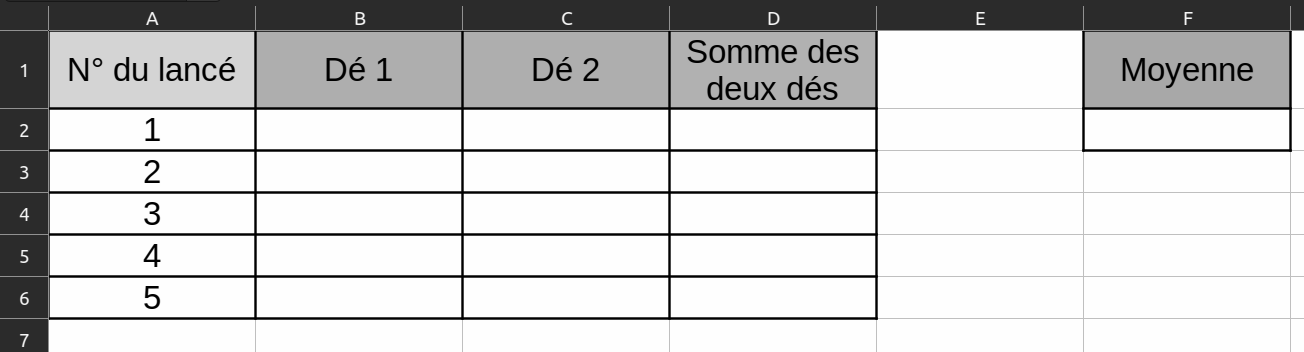
\includegraphics[width=0.7\textwidth]{Images/Tableur, question 1 (gris).png}
	      \end{center}

	      Remplir la cellule \texttt{B2} en utilisant la fonction \texttt{ALEA.ENTRE.BORNES}, puis recopier la formule utilisée dans les cellules \texttt{C2}, \texttt{B3}, \texttt{C3}, ..., \texttt{B6} et \texttt{C6}.
	\item Remplir la cellule \texttt{D2}, de manière à obtenir la somme des deux dés.

	      Étirer cette formule vers le bas afin d'obtenir les cellules \texttt{D3}, \texttt{D4}, \texttt{D5} et \texttt{D6}.
	\item Dans la cellule \texttt{F2}, rentrer une formule permettant de calculer la moyenne des cinq lancés effectués.

	      En appuyant sur la touche \texttt{F9} du clavier, on peut réaliser cinq nouvelles simulations.

	      Quelle est la plus petite moyenne que vous obtenez ainsi ? \correctionDots{qqchose} \\
	      Et la plus grande ? \correctionDots{qqchose}
	\item Afin d'obtenir des résultats plus précis, on veut maintenant simuler $100$ lancés des deux dés.

	      Étendre le tableau pour simuler $100$ lancés, et adapter la formule de la moyenne.
	\item \

	      \begin{minipage}{0.5\textwidth}
		      On veut maintenant créer le tableau ci-contre :

		      Utiliser la fonction \texttt{NB.SI} pour remplir les cellules \texttt{I2} à \texttt{I12}.
	      \end{minipage}\hspace{0.2\textwidth}
	      \begin{minipage}{0.45\textwidth}
		      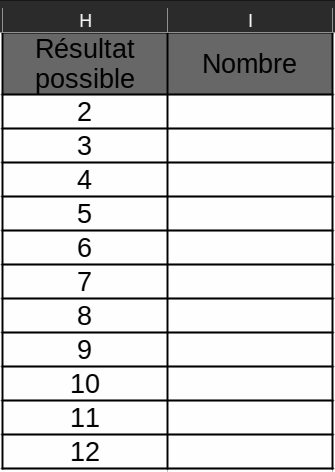
\includegraphics[width=0.4\textwidth]{Images/Tableur, question 4 (gris).png}
	      \end{minipage}

	\item Créer un diagramme représentant le nombre obtenu de chaque résultat :

	      \begin{itemize}
		      \item Dans \texttt{Insertion → Diagramme}.
		      \item Dans la catégorie \texttt{Type de diagramme}, sélectionner \texttt{Colonne}.
		      \item Dans la catégorie \texttt{Plage de données}, sélectionner \texttt{Première ligne en étiquette} et \texttt{Première colonne en étiquette}.
		      \item Appuyer sur \texttt{Terminer} pour créer le diagramme.
	      \end{itemize}

	      Peut-on faire une observation sur ce diagramme ?
	\item Augmenter le nombre de simulations à $500$, et adapter les formules en conséquence.

	      Quelle est alors la forme que prend le diagramme ?
\end{enumerate}

\end{document}